\documentclass{article}
\usepackage{graphicx}
\usepackage{subfig}
\usepackage{amsmath}
\begin{document}
\section{Related Works}
\subsection{Message Authentication}
The purpose of message authentication, marked as MA, is to monitor the integrity of message blocks in the communication. In the scenario of processor-memory communication, MA can be defined as the process to verify that whether "the data read from memory by the processor (or by a specific application) at a given address is the data it last wrote at this address"(\cite{hm_survey}). The on-chip data is assumed to be inaccessible and secure, which is called trusted area; while the data in the transmission and stored in off-chip memory is considered to be accessible to attackers and vulnerable. Transmission path(such as bus) and off-chip memory are called malicious area. 

Figure 1 expresses the concept of MA for processor-memory communication. 
When processor writes a data block, marked as D, to and address, marked as addr, on the memory, processor sends D to MA system and output a message block, marked as message(D, add$_B$), where add$_$b represents and additional data block. The message block message(D,add$_B$) can be the data block D only, D concatenated with a short block(commonly called tag) or other format of D. The content of message(D,add$_B$) is determined by the design of MA system.
When the processor wants to read the data D from address addr, the message(D,add$_B$) is read to SoC and sent to MA system first. After verified by MA, if the data D is not tampered, MA sends a signal indicating pass to processor and send the D to the processor, where D is extracted from message(D,add$_B$) block read from memory.

If the MA finds that the D is tampered, MA sends a failure signal to processor, and invoke the exception handling procedure.
MA system utilizes additional data block in generating message(D, add$_B$). 
\subsection{Evaluating the Security of Message Authentication System}
The purpose of adopting message authentication(MA) system in the system-on-chip is protecting the integrity of the data assessed by processor. 
For new MA system, we expect that it is security first, then behaves good in performance and cost. So it is necessary to form security definition of MA system and do systematical evaluation of security on a new designed MA system.
\subsubsection{Threat Model}
To our knowledge, the attacks aiming to break the integrity of data in malicious area come from two aspects:
\begin{itemize}
	\item Introducing new data: this aspect of attack includes inserting new data block or change content of data block in malicious area
	\item Replacing data block with valid data: this aspect of attack includes replace a data block 
\end{itemize}
\subsubsection{Cryptographic Primitives Adopted in Message Authentication System Design}

As discussed above, the cryptographic primitives adopted in current posted message authentication system are cryptographic hash functions, message authentication code(MAC) functions and added redundancy explicit authentication(AREA). The security of a message authentication system 

\subsection{The Security of a MAC Scheme}
\paragraph{Message Integrity}
In message transmission, the integrity of message means 
\subsubsection{Message Authentication System}
A common way to protect the integrity of message blocks is utilizing message authentication system. Assume the sender A sends message M to receiver B,the message authentication system is eligible to examine the modification on M. The concept of message authentication system is expressed in Figure 1. The sender uses the message as input to the tag generation system(TG$_K$(M)) to generate a short information block called tag. The message is concatenated with tag and transmitted to the receiver. Before the receiver accept the message M, M and its tag T are sent to the verification system(VF$_K$(M,T)). If the output of verification system is 1, that means the M and T are not matched, otherwise the message M is accepted by the receiver. 
\begin{figure}[htbp]
\centering
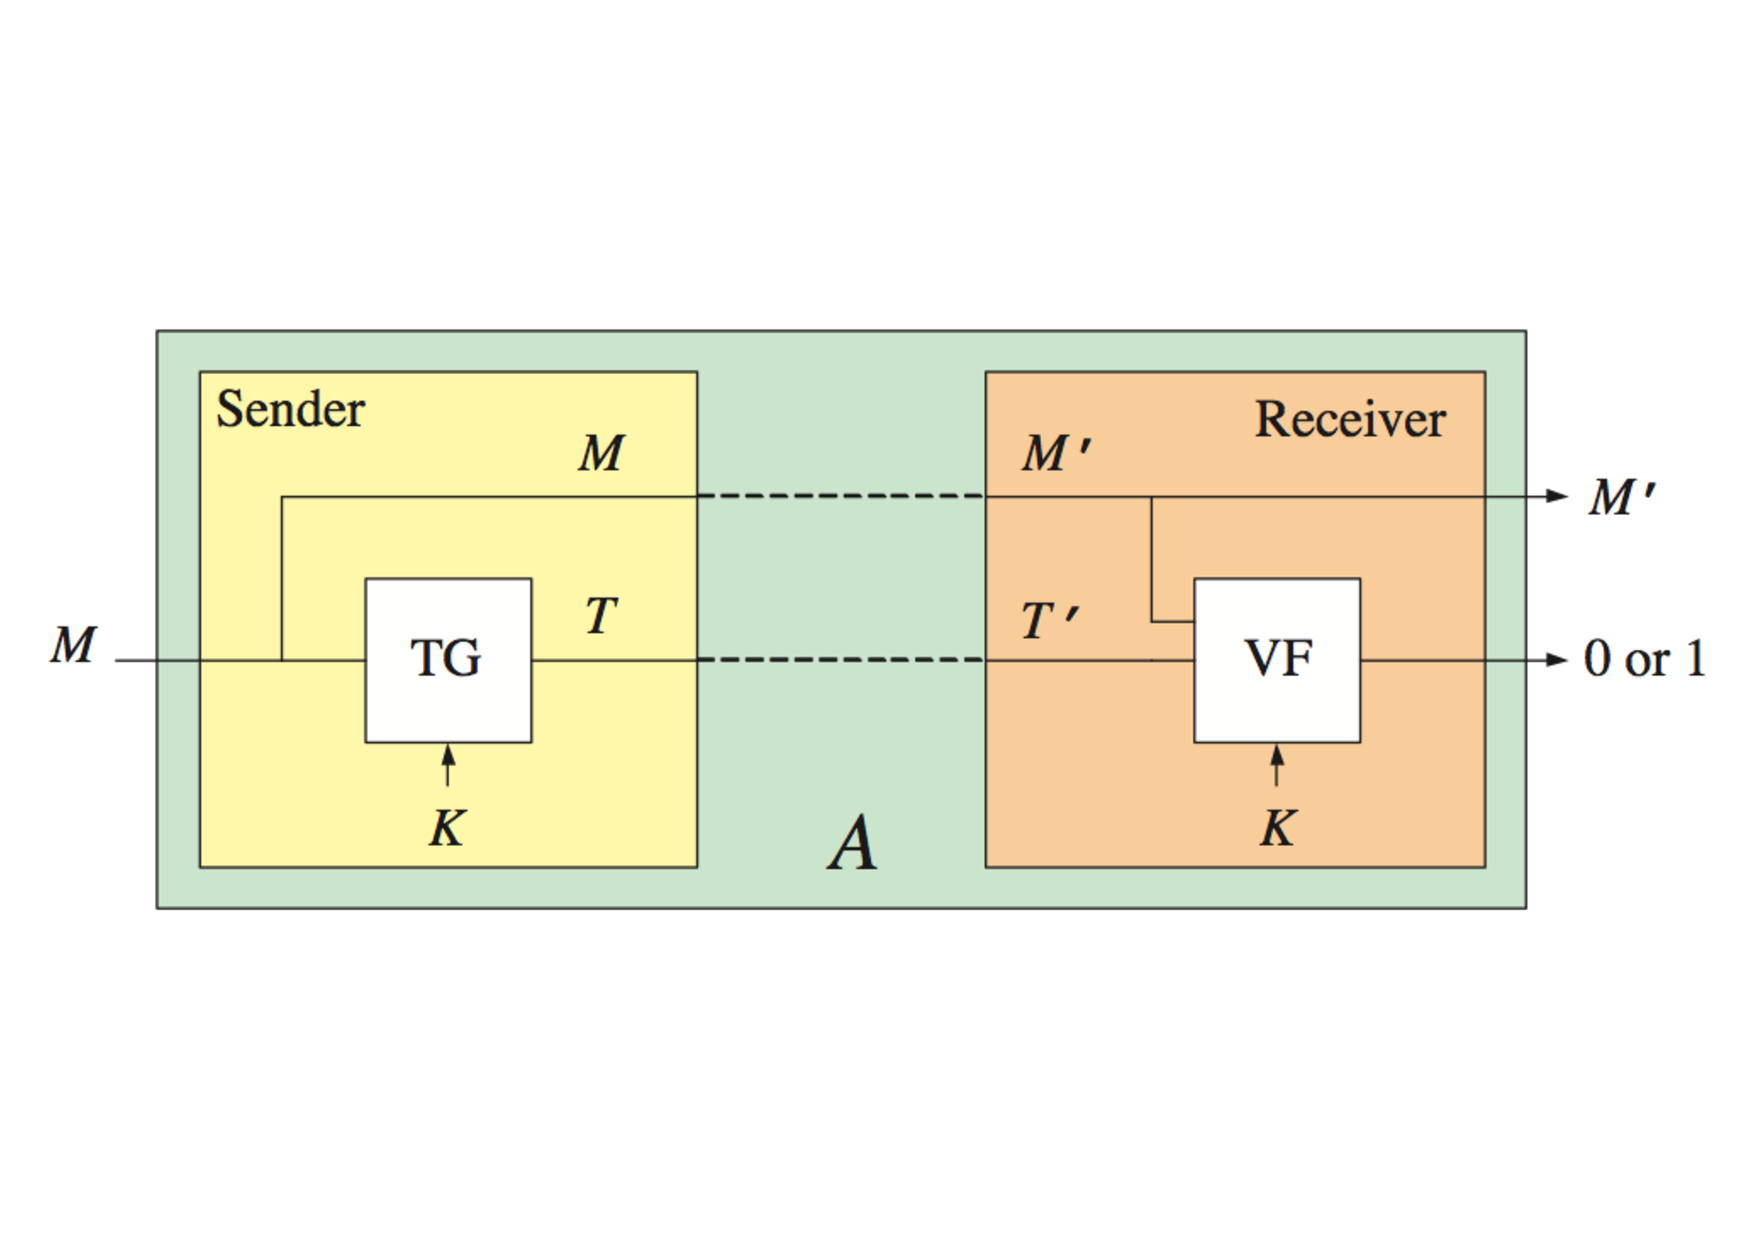
\includegraphics[scale=0.4]{./diagrams/ma.pdf}
\caption{The Concept of Message Authentication System}
\label{fig:1 }
\end{figure}
\paragraph{Common Message Authentication Systems}
The Message Authentication Code(MAC) is a common message authentication system. The concept of MAC scheme can be seen in Figure 2. In a deterministic MAC scheme, the verification system adopts the same key used in tag generation system. In the verification part of a MAC scheme, the tag T1 of message M is computed and compared with the tag T concatenated with the M. If T1=T then the verification system output 1 and the receiver accepts M, otherwise the verification system output 0. 
The early designed MAC schemes are deterministic, which means neither the sender nor the receiver needs to maintain a state used in tag generation. Latter some MAC designs adopt a state maintained by the user in the tag generation, such as the GMAC \cite{gcm} and Cost-Effective Tag Design \cite{cetd}.  

Digital signature is another kind of message authentication system. The signature generation uses a private key while the message verification stage uses public key. The digital signature system can assure non-repudiation of the message protected while MAC schemes can not.
\begin{figure}[htbp]
\centering
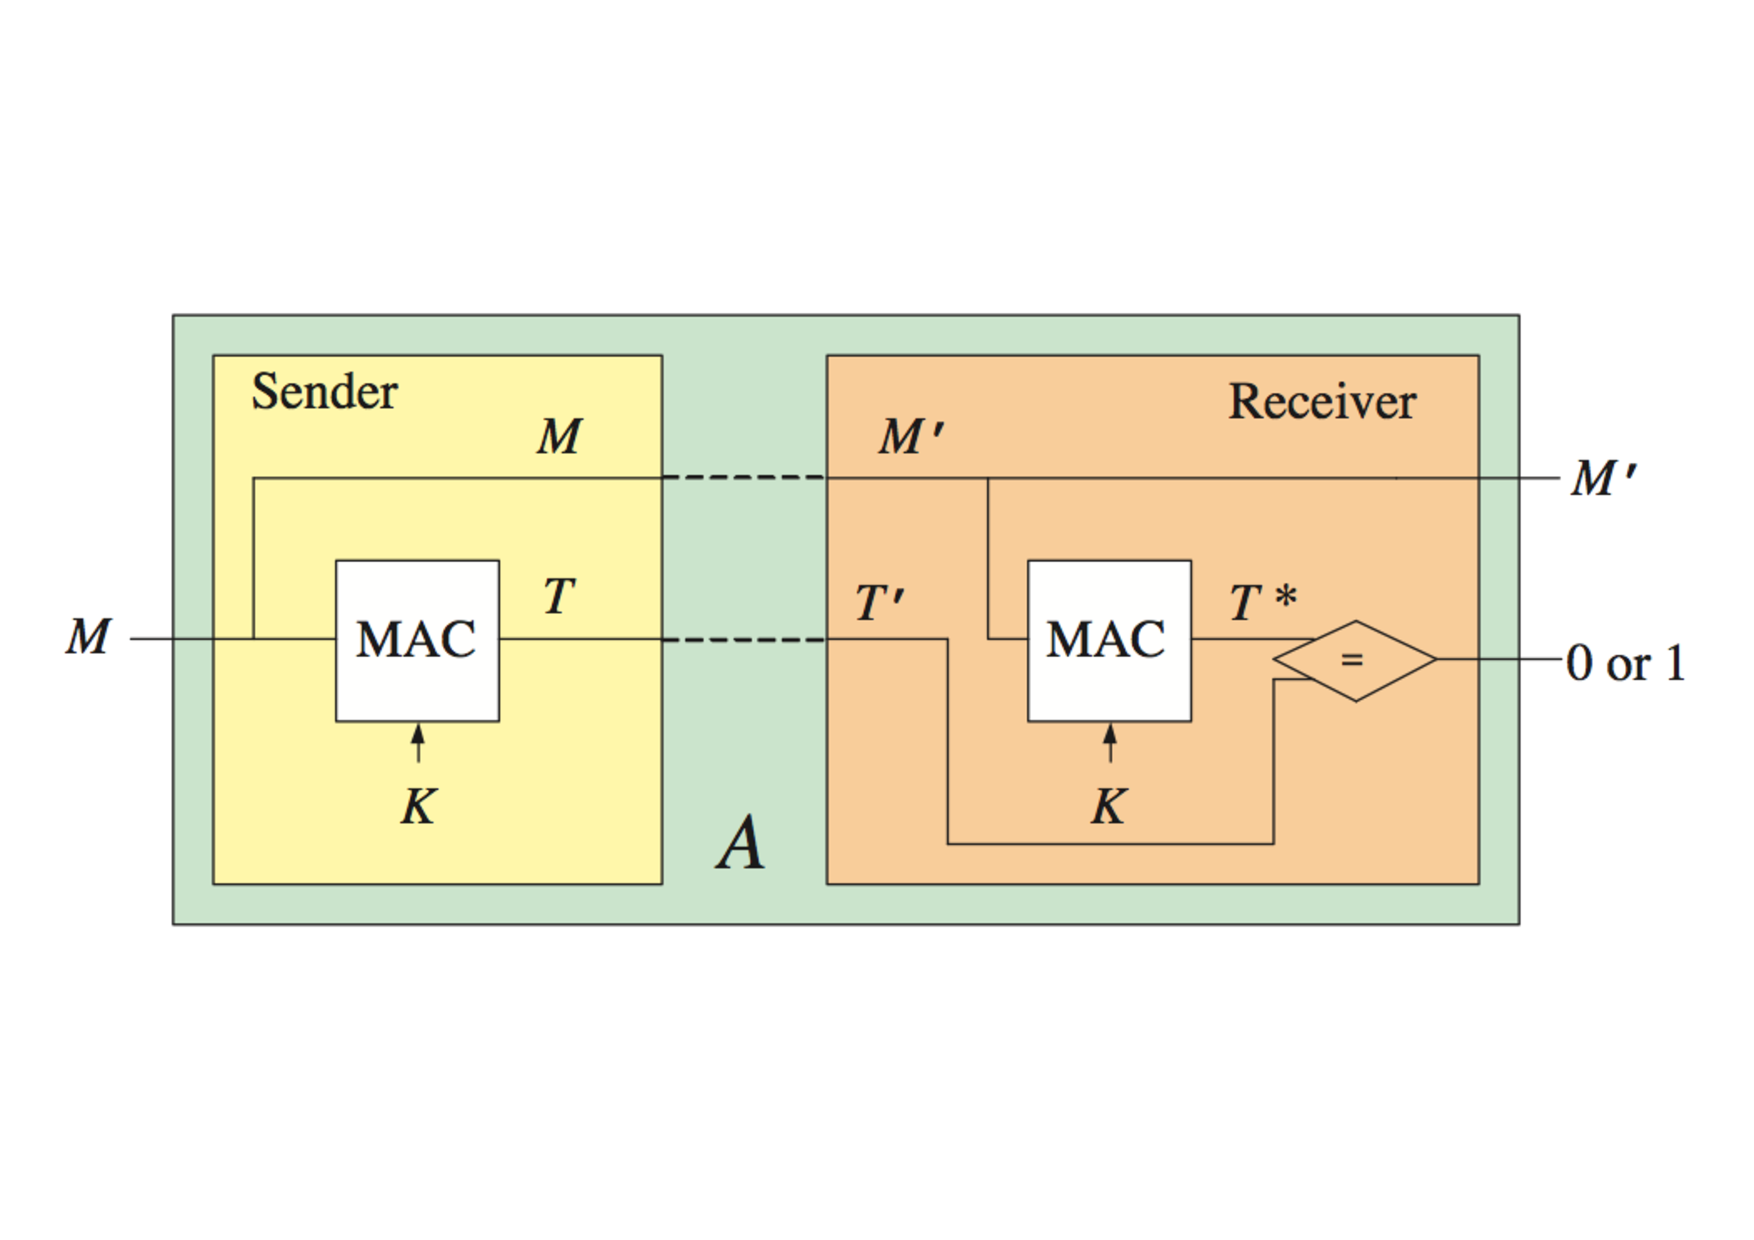
\includegraphics[scale=0.4]{./diagrams/MAC.pdf}
\caption{Message Authentication Code(MAC)}
\label{fig:2 }
\end{figure}
\subsubsection{The Security of MAC schemes}
\paragraph{The forgery attacks}
When attacking a message authentication system, the adversary try to send a pair(M,T) to the receiver to make VF$_k$(M,T)=1 while M did not originate with the legal sender. The fake pair(M$_f$,T$_f$) that makes VF$_k$(M$_f$,T$_f$)=1 is called a forgery from the adversary. A successful forgery attack indicates that the adversary has made a forgery. 
The purpose of a message authentication system is preventing the receiver to accept the message from unauthorized senders, such as an adversary. The quantitative property of a secure message authentication system is the low probability for an adversary to make a successful forgery attack with the limited resource.
\paragraph{Chosen-message attacks}
A strong type of attack that an adversary can conduct on the message authentication system is the adaptive chosen-message attack, marked as uf-cma. When doing uf-cma, the adversary chooses its own input message M and acquires the relative tag T. The adversary try to find the weakness in the design of message authentication system by analyzing the pairs(M,T) of his choice. The uf-cma provides the adversary with the most capability to succeed in the forgery attack. The probability that an adversary conducts a successful forgery attack after limited times of uf-cma is adopted as the basic quantitative security property of a message authentication in cryptography. This fact was also mentioned in \cite{Rogaway2011}.
\paragraph{The Security Notions of MAC schemes}
The formalised quantitative notion of the security of a MAC scheme was introduced by Bellare et al. in \cite{cbc1994}. This notion follows the security notion of digital signature introduced in \cite{signature}. The successful forgery on a MAC scheme from an adversary A is measured by a experiment called Forgery(MAC,A). In Forgery(MAC,A),  
the adversary A is provided a black-box access to the tag generation system TG$_K$(). When TG$_K$() takes an input message M$_i$, it returns tag T$_i$ to A. A conducts uf-cma by keep sending the message queries M$_i$ and observes the relative tag T$_i$ for limited times. On the other hand, A is provided a black-box access to the verification system VF$_K$(). When A sends a pair(M$_j$,T$_j$) to VF$_K$(), the VF$_K$() computes the tag T of M$_j$ and compares T with T$_j$. If T=T$_j$ then VF$_K$()=1 otherwise 0. If A sends a pair(M,T) that makes VF$_K$() outputs 1 while M has not appeared in the previous queries of uf-cma, then A succeeds a forgery attack and Forgery(MAC,A)=1.

The quantitative security notion of a MAC scheme is forgery probability, expressed as Forgery$_MAC$=Pr[Forgery(MAC,A)=1].
\paragraph{The Correlation between Security and Randomness}
Goldreich, Goldwasser, and Micali asserted in \cite{prf} that any good pseudorandom function(PRF) is a secure MAC scheme under the quantitative security notion. Bellare, Kilian and Rogaway proved this assertion in \cite{cbc1994} saying that if a system behave like a pseudoranom function, this system is a secure MAC scheme if meeting the requirements on domain and range of MAC schemes. Based on these two reduction of security notion, latter researches on security evaluation of MAC schemes posted their focuses on analyzing whether the MAC scheme evaluated behaves like a PRF.
\paragraph{The Randomness of a MAC scheme}
The definition of PRF was introduced in \cite{prf} indicating that PRF could not be distinguished from a ideal random function each bit of whose output was a coin flip. To define how closely a MAC scheme behaves like a PRF, Bellare et al. provided a quantitative notion in \cite{cbc1994} named Adv$^{PRF}_{MAC}$(), which was based on the concept of distinguisher introduced in\cite{prf}. 

Let F$_0$ and F$_1$ be two function with a common domain D and a common range R. A distinguisher A for F$_0$ versus F$_1$ is an adverary A that has access to a black box named oracle f:D->R. After accessing the oracle f, A computes a bit. Assume the function stored in the oracle f is X and A guesses that X is in the oracle, then A computes 1 otherwise 0. The the advantage of A in distinguishing F$_0$ from F$_1$ is expressed as Adv$^{F0}_{F1}$=Pr[f$\stackrel{R}{\longleftarrow}$F0:A$^{F0}$=1]-Pr[f$\stackrel{R}{\longleftarrow}$F1:A$^{F1}$=1]. Pr[f$\stackrel{R}{\longleftarrow}$F0:A$^{F0}$=1] means when the content of oracle f is F0, A guesses that F0 is in oracle then output 1.

We can see that if F0 behaves much like F1, it is hard for A to distinguish between F0 and F1 then Adv$^{F0}_{F1}$ is very small. This case is adopted by Bellare et al. in the quantitative notion of randomness of a MAC scheme. If the randomness of a MAC scheme is good, then the MAC scheme behaves like a PRF and Adv$^{[PRF]}_{MAC}$ is small. 
\subsection{Implementation of Tag Design}
\subsubsection{Network and Cloud System}
\subsubsection{Memory Protection}
\paragraph{Single-processor System}
\paragraph{Multiple-processor System}
\subsubsection{Crypto-hardware Design}
\subsection{Security Evaluation of Tag Design}
\end{document}